\section{Algebraic Multigrid} \label{sec_amg}
\subsection{Introduction}
As mentioned earlier, the most common way to solve a SPD system is to use
conjugate gradient preconditioned with SSOR (PCG-SSOR). In this research, we
will compare the calculation time using PCG-SGS, which is a particular version
of PCG-SSOR, with the time needed by CG 
preconditioned with an algebraic multigrid method. In \cite{amg_pn}, the authors 
used an algebraic multigrid method to precondition the Krylov solver for the 
even-parity finite element-spherical harmonics (FE-$P_N$) method. The AMG 
preconditioner resulted in a 60\% reduction in the solution time compared to 
ILU(0) preconditioning and even more reduction compared to SSOR preconditioning. 
Rather than writing our own AMG code, we will be testing the ML package 
\cite{ml_guide} from the Trilinos library and the AGMG code \cite{agmg_guide}. 
ML is a multigrid preconditioning package that uses a smoothed aggregation 
algebraic multigrid to build a preconditioner for a Krylov method. AGMG is an 
aggregation-based algebraic multigrid code written in Fortran 90.

The first multigrid methods developed were geometric multigrid used as 
stand-alone solvers. In many applications, they achieve the so-called 
``textbook multigrid efficiency'', i.e. ``the solution to the governing 
system of equations [is attained] in a computational work that is a small 
multiple of the operation counts associated with discretizing the system'' 
\cite{textbook_eff}. However, in many other applications, multigrid methods, 
and particularly algebraic multigrid methods, cannot achieve such efficiency 
\cite{k_cycle} and in such cases, they are often used as preconditioner for 
Krylov subspace methods. 

Before solving a system of equations with a general multigrid method, we
explain how to solve it using a two-grid method. We want to
solve the following system:
\begin{equation}
  \bs{A}_f u_f = b_f
\end{equation}
define on the grid $\Gamma_f$. The two-grid algorithm is given by :
\begin{enumerate}
  \item $\nu_1$ pre-smoothing iterations using a smoother (Jacobi,
    Gauss-Seidel or ILU) and an initial guess $u_0$: $u = S^{\nu_1}(u_0,b_f)$
  \item Compute the residual on the fine grid $\Gamma_f$ and restrict it to
    the coarse grid $\Gamma_c$: $r_c = \bs{R}(b_f-\bs{A}_f u)$
  \item Solve the system on the coarse grid: $v=\bs{A}_c^{-1} r_c$
  \item Interpolate the coarse grid correction to the fine grid and add the
    correction to $u$: $u=u+\bs{P}v$
  \item $\nu_2$ post-smoothing iterations: $u = S^{\nu_2}(u,b_f)$
\end{enumerate}
When using AMG, the matrix $\bs{A}_c$ on the coarse grid is given by the
Galerkin approximation:
\begin{equation}
  \bs{A}_c = \bs{R} \bs{A}_f \bs{P}
\end{equation}
where $\bs{P}$ is a prolongation matrix and $\bs{R}$ is a restriction matrix. 
Solving the system $\bs{A}_c v = r_c$ on the coarse grid is generally very
expansive, therefore this step is recursively replaced by $\gamma$ two-grid
methods until the system can be efficiently inverted with a direct solver.
This yields the multigrid method. When $\gamma = 1$, respectively $\gamma =
2$, the multigrid method is said to use a $V-$cycle, respectively a $W-$cycle: 
\begin{figure}[H]
  \centering
  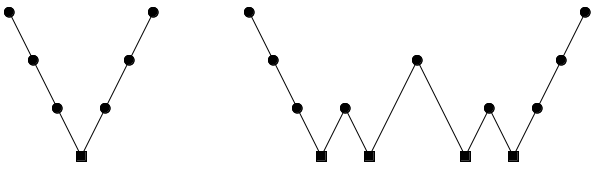
\includegraphics[width=0.5\textwidth]{v_w_cycles}
  \caption{$V-$ and $W-$cycles.}
\end{figure}
A dot represents a smoothing operation and a square a direct inversion. The
grid transfer operators are symbolized by lines.

The main difference between geometric and algebraic multigrid is in the method
to coarsen the grid. Algebraic multigrid methods only use the properties of the
matrix. Among the algebraic multigrid methods, there are three main different 
types: the classical Ruge-Stueben AMG, the plain aggregation AMG, and the
smoothed aggregation AMG. ML uses smoothed aggregation AMG and AGMG
uses plain aggregation AMG. Next, we briefly explain the coarsening step in
ML and AGMG. The coarsening step is the most important 
step because if the coarsening is too fast, the convergence rates will 
decrease. However, if the coarsening is too slow, a lot of memory may be 
required to solve the problem. 

\subsection{ML}
When using a smoothed aggregation scheme, the smoothed interpolation operators,
$\bs{P}_k$, are the transpose of the coarsening operators,
$\bs{R}_k=\bs{P}_k^T$. Therefore, when the $\bs{P}_k$ are built, the
coarsening is known. First, the graph of the matrix is constructed: if the element
$(i,j)$ or $(j,i)$ of the matrix is non-zero, an edge is built between the
vertex $i$ and the vertex $j$ \cite{ml_guide}. Second, the vertices are
aggregated. When using ML on a single processor, two aggregation schemes can
be used: the uncoupled scheme or the maximally independent sets (MIS) scheme. 
The uncoupled scheme tries to build aggregates of size $3^d$ where $d$ is the
dimension of the problem. The algorithm works as follows \cite{mis}:
\begin{description}
  \item[Step 1:] As long as there are points not adjacent to an aggregate:
    \begin{enumerate}
      \item Choose a point which is not an adjacent to an
        aggregate. This point is a new root point.
      \item Define a new aggregate as the root point and its neighbors 
    \end{enumerate}
  \item[Step 2:] Add all the points left to the existing aggregates or form a
    new aggregates with them
\end{description}
The MIS scheme used in ML applied the MIS algorithm \cite{graph_coloring} to
the graph produced by the square of the matrix $\bs{A}$. These two coarsening 
schemes use a fixed ratio of coarsening between levels. 

Once the aggregation is done, a tentative prolongator matrix, $\bs{\tilde{P}}_k$ 
is constructed \cite{mis}. A example of $\bs{\tilde{P}}_k$ is given by:
\begin{equation}
  \bs{\tilde{P}}_k(i,j) = \left\{
  \begin{aligned}
    &1 &\textrm{if }i^{th}\textrm{ point is contained in }j^{th}\textrm{
    aggregate}\\
    & 0 &\textrm{otherwise}
  \end{aligned}
  \right.
\end{equation}
This tentative prolongator could be used as prolongator but smoothing it
allows to have a more robust scheme. Let $\bs{S}_k$ be a smoother, for example
damped Jacobi, the prolongator matrix is given by:
\begin{equation}
  \bs{P}_k = \bs{S}_k \bs{\tilde{P}}_k
\end{equation}

\subsection{AGMG}
Unlike ML, in AGMG the prolongator is not smoothed which results in a
cheaper setup and a decrease of required memory \cite{agmg2}. However, as
explained previously, the scheme is less robust. To counteract this weakness, the
aggregation scheme is more complicated. Coarsening algorithms which control
the size of the aggregates tends to produce a few badly shaped aggregates.
Since the convergence of AMG is bounded by the worst aggregate, even a small 
number of badly shaped aggregates can have a huge impact on
the convergence. In AGMG, the aggregation algorithm has as input the upper
bound of the two-grid condition number. When the aggregates are constructed,
their quality is checked. Obviously, this increases the cost of the coarsening
and it is therefore important that the coarsening is fast enough. Since the 
algorithm does not control the size of the aggregates, it is difficult to 
control the speed of the coarsening. However, controlling the condition number
is much more interesting than controlling the coarsening speed. If the algorithm 
controls the condition number, it will not create bad aggregates but instead, it 
may create a few aggregates below the target size. This obviously 
does not affect the efficiency of the method in an noticeable way \cite{agmg2}. 
In AGMG, the aggregation is done by a few passes of a pairwise aggregation 
algorithm which allows the computation of the aggregate quality to remain very 
simple and to keep the cost per iteration low. The advantage of controlling the 
condition number becomes even more important when a $K-$cycle or Krylov-cycle is 
used instead of the more common $V-$ or $W-$cycles. The difference between the 
$K-$cycle and the $V-$ or $W-$cycle is that the $K-$cycle uses recursively a 
few iterations of a Krylov solver preconditioned by a coarser grid to solve 
the coarse grid problem in the two-grid algorithm \cite{k_cycle}. This scheme 
is nonlinear and requires, when the system is SPD, to use flexible CG 
\cite{fcg,fcg_2,fcg_3,fcg_4} as Krylov solver. The advantage of the $K-$cycle is 
an increased robustness compared to $V-$ and $W-$cycle. Even when the condition 
number of the two-grid method is large, the convergence properties of the 
$K-$cycle can be independent of the number of levels \cite{k_cycle}. The 
computational cost of $K-$cycle is about the same than the cost of the 
$W-$cycle. If the number of unknowns does not decrease sufficiently from one 
level to the next, the $K-$cycle at one level is replaced by a $V-$cycle at 
this same level.
